\documentclass[12pt, a4papre]{article}
\usepackage[catalan]{babel}
\usepackage[unicode]{hyperref}
\usepackage{amsmath}
\usepackage{amssymb}
\usepackage{amsthm}
\usepackage{xifthen}
\usepackage{listings}
\usepackage{float}
\usepackage{siunitx}
\usepackage{graphicx}
\usepackage{indentfirst}

\newcommand{\norm}[1]{\lvert #1 \rvert}
\graphicspath{ {./Images/} }

\hypersetup{
    colorlinks = true,
    linkcolor = blue
}

\author{Daniel Vilardell}
\title{Previ practica 3}
\date{}

\begin{document}
	\maketitle
	
	\textbf{Qüestió 1:} Tenint en compte que la ona ha d'anar i tornar el TOF sera el seguent:
	
	Per una distancia $d = 50cm$ tenim $TOF = \frac{1}{340} = 2.94ms$ i per una distancia $d = 2m$ tenim $TOF = \frac{4}{340} = 11.7ms$.
	
	\textbf{Qüestió 2:} Cuan simulem amb PSpice el circuit proposat obtenim per a la senyal d'entrada vermella la envolvent blava i veiem que funciona be.
	
	\begin{figure}[H]
		\begin{center}
		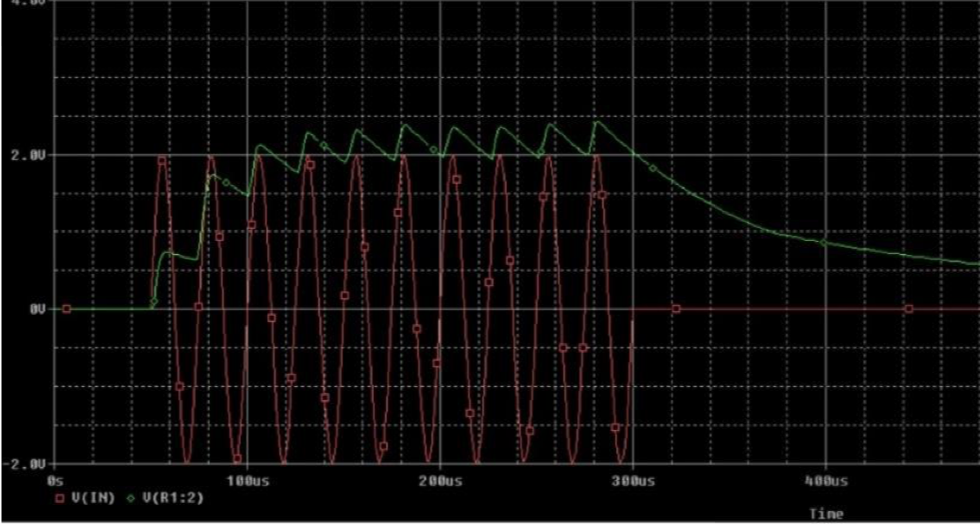
\includegraphics[width=110mm]{previ_4_1.png}
		\end{center}
	\end{figure}
	
	\textbf{Qüestió 3:} Analitzem primer el circuit considerant saturació positiva, es a dir que $V_o = V_{cc}$.
	
	\[
		V_p = \frac{R_7}{R_6 + R_7}V_i+\frac{R_6}{R_6 + R_7}V_0 \qquad V_n = \frac{V_{cc}}{2}
	\]
	\[
		\frac{R_7}{R_6 + R_7}V_i+\frac{R_6}{R_6 + R_7}V_{cc} >  \frac{V_{cc}}{2} \implies V_i > 5.802V
	\]
	
	Per altra banda analitzem el circuit per la saturació negativa, es a dir amb $V_o = 0V$
	
	\[
		V_p = \frac{R_7}{R_6 + R_7}V_i \qquad V_n = \frac{V_{cc}}{2}
	\]
	\[
		\frac{R_7}{R_6 + R_7}V_i < \frac{V_{cc}}{2} \implies V_i < 6.198V
	\]
	
	Per tant tenim que $5.802V < V_i < 6.198V$.
	
	\begin{figure}[H]
		\begin{center}
		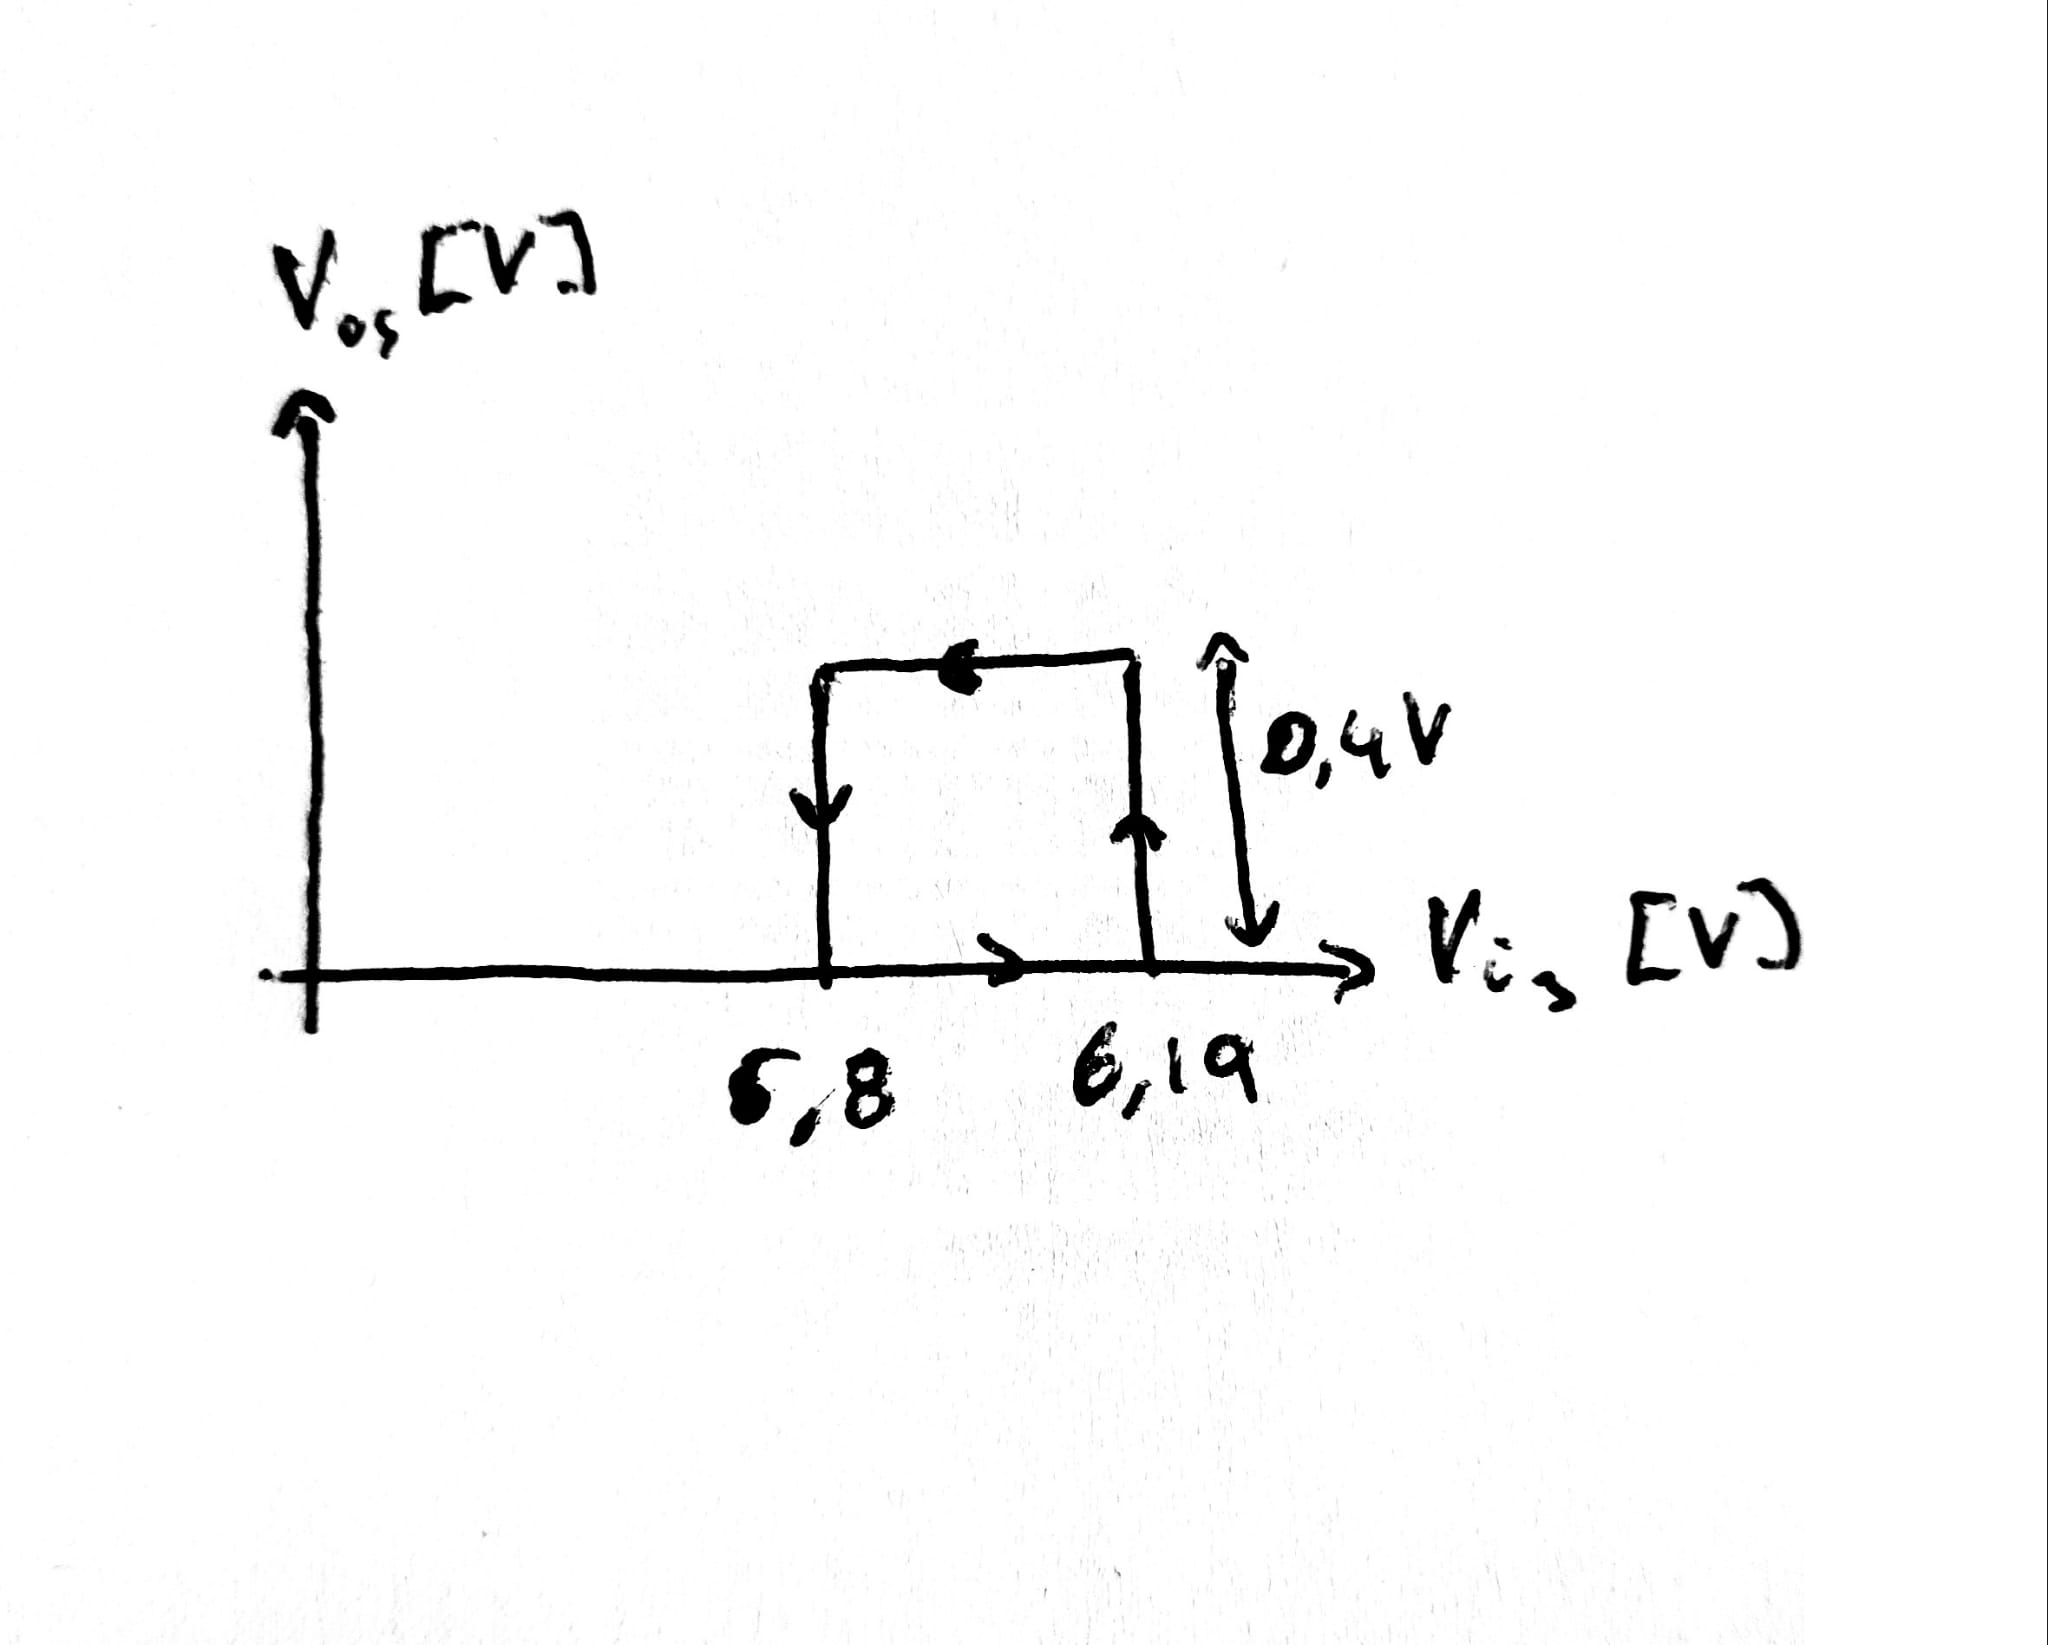
\includegraphics[width=80mm]{previ_4_1_2.jpeg}
		\end{center}
	\end{figure}
	
	
\end{document}




